In rare occasioni vediamo \textit{violazioni} di leggi di conservazione, che sono valide solo per interazione forte ed elettromagnetica. Queste sono note come \textit{interazioni deboli} (w.i.) a causa della loro piccola costante di accoppiamento. L'interazione debole avviene in quasi tutti i processi ma il loro effetto è trascurabile, eccetto nei casi in cui tutto il resto è proibito (e.g. decadimenti che violano la stranezza, charm,\dots). A causa della interazione forte, la materia \textit{stabile} è formata solo da $u,d,e^-$. Gli altri quark e leptoni carichi sono instabili e decadono debolmente. Dunque nonostante la loro "debolezza" (piccolo range di interazione $10^{-3}$ fm e piccole sezioni d'urto $10^{-47}$ m$^2$), l'interazione forte assume un ruolo fondamentale nel determinare il nostro mondo.\\
\textit{Tutte} le particelle elementari, eccetto gluoni e fotoni (mediatori dell'interazione), vedono l'interazione debole: i quark ed i leptoni carihi interagiscono debolmente, i neutrini interagiscono \textit{solo} debolmente. Per questo motivo la nostra conoscenza dell'interazione debole, almeno fino agli anni 70, si ottenne solo da decadimenti di particelle (e.g. $\pi^+$ e $\mu^+$ che decadono) e da fasci di neutrini.
\subsubsection{Piccolo ripassino}
Rivediamo i tempi di vita media di alcuni decadimenti:
\begin{alignat*}{3}
    &\Delta^{++} \to p\pi &&\sim 10^{-23}s &&\textnormal{int. forte} \\
    &\Sigma^0\to\Lambda\gamma &&\sim6\cdot10^{-20}s \textnormal{ }&& \textnormal{int. e.m. (c'è un }\gamma) \\
    & \pi^0\to\gamma \gamma &&\sim 10^{-16}s && \textnormal{int. e.m. (ci sono due }\gamma)
\end{alignat*}
\begin{align*}
    & \begin{aligned}
       & \Sigma\to n\pi &&\sim10^{-10}s \\
       & \pi^-\to\mu\nu_\mu&&\sim10^{-8}s \\
       & \mu^-\to e^-\bar\nu_e\nu_\mu&&\sim10^{-6}s \\
       & n\to pe^-\bar\nu_e&&\sim15\textnormal{ min}
    \end{aligned}
     \left.\vphantom{\begin{matrix}
    \text{Equazione 7}\\
    \text{Equazione 8}\\
    \text{Equazione 9}\\
    \text{Equazione 10}
    \end{matrix}}\right\} \text{int. debole}
    \end{align*}
\begin{itemize}
    \item Dobbiamo spiegare l'enorme intervallo di tempi di vita media che va da $10^{-12}$ s a 15 min.
    \item L'interazione debole è anche caraterizzata da sezioni d'urto estremamente piccole \\
    ($\sim10^{-39}cm^2=1$ fb)
    \begin{alignat*}{3}
    &\sigma(\nu_\mu+N\to N+\pi+\mu)&&=10^{-38}\textnormal{cm}^2(10\,\textnormal{fb}) &&\textnormal{ ad 1 GeV}\\
    &\sigma(\pi+N\to N+\pi)&&=10^{-26}\textnormal{cm}^2(10\,\textnormal{mb}) &&\textnormal{ ad 1 GeV}
    \end{alignat*}
    \item L'interazione debole viola molte leggi di conservazione: parità, coniugazione di carica, stranezza, etc.
    \item Come già detto, a causa della loro debolezza, l'interazione debole può essere osservata nella materia ordinaria solo nel decadimento $\beta$, perché non da origine ad alcun stato legato. Tuttavia, sono la base del funzionamento delle stelle che senza di essa non esisterebbe:
    \begin{equation*}
    p+p\to d+e^++\nu_e
    \end{equation*}
\end{itemize}
\subsubsection{Corrente carica e corrente neutra}
Nel modello standard, l'interazioni deboli sono classificate in due tipologie, in base ai loro portatori di carica:
\begin{itemize}
    \item \textbf{Correnti cariche (CC)}, scambio di $W^\pm$: nei processi CC, la carica dei quark e leptoni cambia di $\pm1$; allo stesso tempo c'è una variazione della loro identità, cioè del flavour, secondo la teoria di Cabibbo.
    \begin{figure}[H]
        \centering
        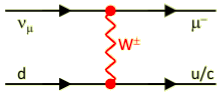
\includegraphics[width=0.5\textwidth]{immagini/fig_cc_process.png}
        \caption{Processo di corrente carica. Un $d$ emette $W^-$ e diventa $u$.}
        %\label{fig:cc_process}
    \end{figure}
    \item \textbf{Correnti neutre (NC)}, scambio di $Z$: in questo caso i quark ed i leptoni restano invariati (non c'è FCNC Flavour-Changing Neutral Current). Fino al 1973 nessun processo NC fu osservato, anche se un esempio evidente lo abbiamo ossia il $\gamma$ della interazione elettromagnetica non porta alcuna carica.
    \item Negli anni 60 Glashow, Salam e Weinberg (e molti altri teorici) svilupparono una teoria, oggi parte del Modello Standard, che unifica la interazione debole (sia CC che NC) e l'elettromagnetismo.
    \item Il Modello Standard fu ideato \textit{prima} della scoperta di NC e del suo portatore (bosone $Z$), predetto dal Modello Standard negli anni 60 e direttamente osservato al CERN nel 1983.
\end{itemize}
\subsubsection{Classificazione}
\begin{minipage}{0.6\textwidth}
    \begin{figure}[H]
        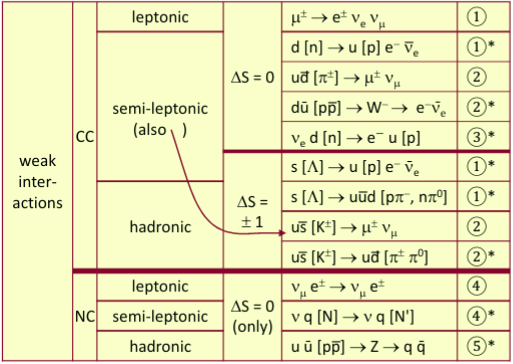
\includegraphics[width=\textwidth]{immagini/fig_table_weak_int.png}
        %\caption{Tabella delle interazioni deboli.}
        %\label{fig:table_weak_int}
    \end{figure}
    Nell'ultima colonna l'asterisco indica che l'adrone interagente, mostrato tra le parentesi quadre, è composto. Nei diagrammi ci sono solo i quark interagenti. Gli altri partoni spettatori non partecipano alla interazione.
\end{minipage}
\begin{minipage}{0.30\textwidth}
\begin{figure}[H]
    \centering
    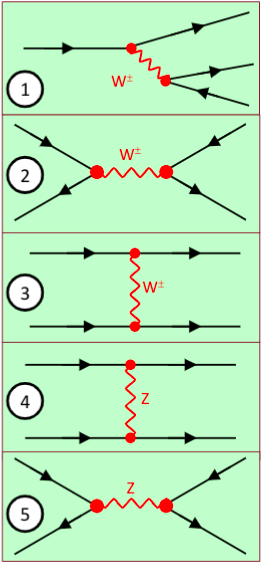
\includegraphics[width=\textwidth]{immagini/fig_xchange_bosons.png}
    %\caption{Scambio di bosoni nell'interazione debole.}
    %\label{fig:xchange_bosons}
\end{figure}
\end{minipage}
